% !TeX root = ../main.tex

\chapter{绪论}

\section{研究背景及研究意义}
\par 近年来,信息技术及人工智能技术已经渗透到我们生活的方方面面,我们幻想的上个世纪许多存在于科幻小说中的内容已经成为现实:如人工智能 AlphaGo 算法击败了人类顶尖的棋手,生产线上大批量的机器人和机械臂取代了人工。
相信不久的将来,大众乘坐宇宙飞船进行星际旅行的梦想将会成为现实。

\par 在制造业领域,工业4.0和智能制造正在产生着新一轮的技术变革。在上海的特斯拉超级工厂,大量的自动化、智能化的设备正在24小时不间断工作,极大地提高了生产效率。
德国的西门子公司也利用工业4.0的理念,将传统的生产线升级为完全自动化、可自主学习的智能生产线。阿里巴巴的“新制造”理念,借助数据和AI技术,打造了一条灵活、智能的供应链,能快速响应市场需求,实现个性化生产。

\par 在众多人工智能领域中,智能机器人无疑是近年来备受关注的领域之一。2021年前11个月,全国有316个机器人项目获得融资,总金额超过330亿人民币。
刚刚过去的北京冬奥会,实现了奥运史上首次利用自动驾驶技术控制无人车的火炬接力、运动员接驳、物资配送(如图\ref{fig:peking}所示)、自动清扫等自动化服务,近百台不同类型的自动驾驶车辆安全有序地运行,既保障了北京冬奥会在复杂天气与疫情的双重挑战下顺利举行,又用实际行动将科技冬奥的主题展现得淋漓尽致。
在我国某大型房地产开发商的建筑工地上\cite{jiqirenjianzhu_chuangxin,jiqirenjianzhu_hulian},上百台不同类别的智能建筑机器人正如火如荼地进行着各项工作。
其中,喷涂机器人可以避免建筑工人在喷涂过程中带来的粉尘职业病和高空作业风险。如图\ref{fig:grinding}所示,地坪研磨机器人可以在建筑物顶层全露天、无遮挡地,进行地面研磨工作,只要用上激光测量,就可以让刮板保持在毫米级的精度,即可以为后续的抛光、铺地板等工作打下高质量的基础,又将建筑工人从这个工地上最辛苦的工作中解放出来。

\begin{figure}[htb]
	\centering
	\begin{minipage}[t]{0.45\linewidth}
		\centering
		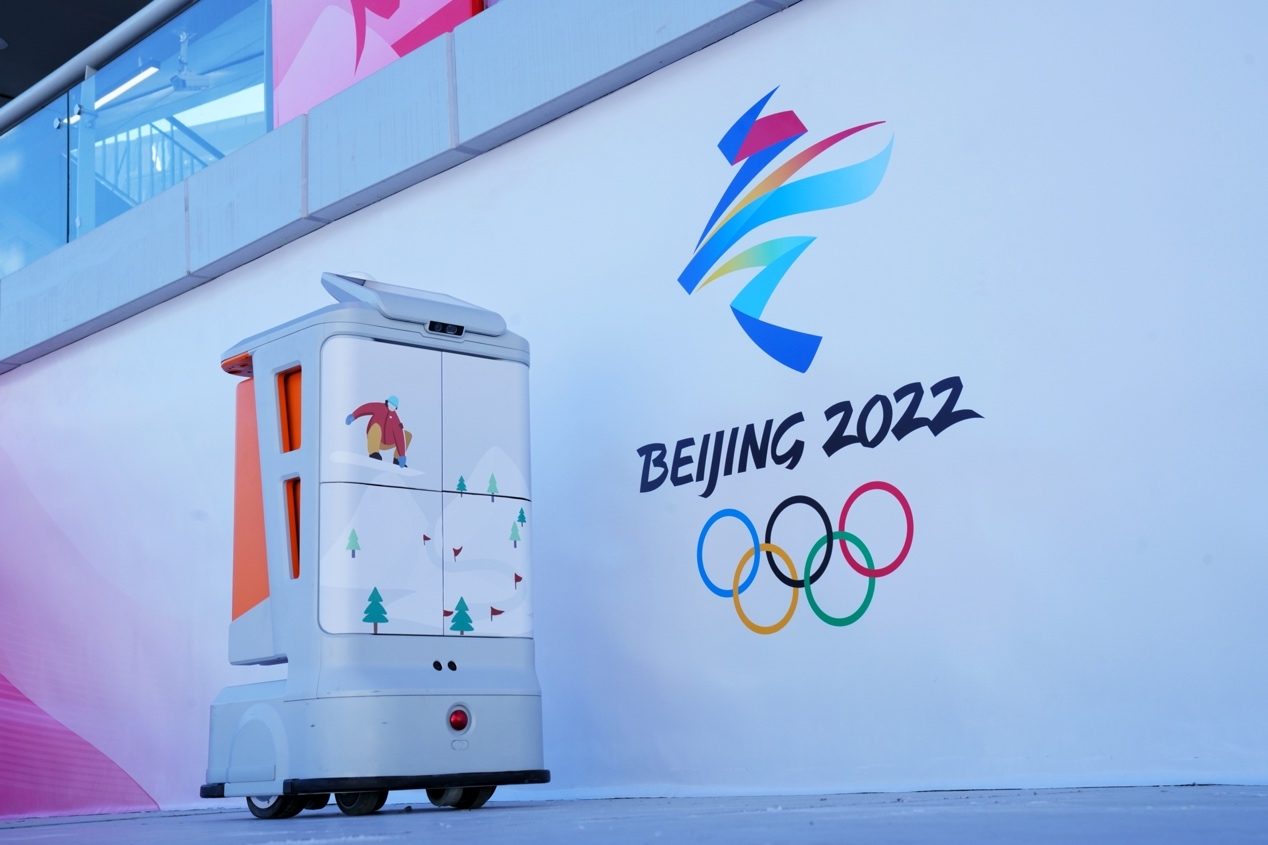
\includegraphics[height=4.5cm,keepaspectratio]{figures/delivery_robot.jpg}
		\caption{北京冬奥会配送机器人}
		\label{fig:peking}
	\end{minipage}
	\begin{minipage}[t]{0.45\linewidth}
		\centering
		\includegraphics[height=4.5cm,keepaspectratio]{figures/floor_grinding_robot.jpg}
		\caption{地坪研磨机器人}
		\label{fig:grinding}
	\end{minipage}
\end{figure}

\par 然而,智能机器人技术仍然面临巨大的挑战及发展空间。在自动驾驶领域,随着技术级别从L2(部分自动驾驶)到L3(有条件的自动驾驶)、L4(高度自动驾驶)级别\cite{unifiedAV}的迈进,其决策系统对感知技术的要求已经不能再局限于二维图像识别和几何模型重建,还需要对周围物体进行实时语义分割,需要在单位时间内处理数量更多、尺寸更大、信息更复杂的全景分割图像\cite{panopticsegmentation,electronics10161960},并实时转换成包含语义信息和实例信息的三维模型。
由于诸多技术的约束,现有的自动驾驶系统只能在天气晴朗、道路交通环境简单的情况下短暂地解放驾驶员的双手\cite{s21165397}。
在上述房地产开发商的建筑工地上,其喷涂机器人只能处理固定的场景,加上机械臂宽度限制和运动时产生的距离误差,每次只能固定在一个地点进行喷涂,然后由人工搬运到另一个地点继续喷涂,不仅使建筑工人消耗大量体力,而且喷涂不够均匀,工作成后仍然需要人工再次修理,产生事倍功半的效果\cite{MANUELDAVILADELGADO2022101787}。

\par 根据上述对智能机器人技术所面临挑战的分析,可以得出结论:如何对重建出的模型进行实时语义分割,是三维重建领域目前面临的关键问题;
如何对动态范围场景进行增量式重建,以及如何提高三维重建及语义分割的速度,快速响应输入的数据,是制约智能机器人大规模应用的重要问题。
这些问题亟需学术及工业界投入大量的人力、资金成本对其进行研究、改进和实践。

\par 针对上述问题,本论文将致力于开发一个基于RGB-D相机的实时三维重建及语义分割系统,输入相机在运动过程中捕获的RGB图像和深度图像,经过预处理后生成相机位姿矩阵和像素级别的语义分割图像,并且利用这些信息对真实世界场景进行实时三维重建及语义分割,转换成包含RGB信息和语义信息的点云模型,并将其重建过程和结果进行可视化展示。

\par 通过使用该实时三维重建及语义分割系统,可以提高智能机器人在各种场景下的适应性和工作效率,为推动智能机器人的广泛应用和产业发展作出贡献。

\section{国内外研究现状}

\subsection{RGB-D 相机}

% \subsubsection{简介}
\par RGB-D(Red Green Blue-Depth)相机是一种深度感知设备,它能够捕捉RGB图像以及与之对应的深度信息,主要有结构光(Structured
Light)\cite{structuredlight}和飞行时间(Time Of Flight, ToF)\cite{timeoflight}两种工作原理。
截至目前,RGB-D相机在许多领域都得到了广泛的应用:

\paragraph{三维重建}
\par RGB-D相机为三维重建提供了详细的场景信息,包括物体的形状、纹理和距离。这使得RGB-D相机在实时建模、室内建筑物扫描以及增强现实(Augmented
Reality, AR)和虚拟现实(Virtual Reality, VR)等领域具有广泛应用\cite{kim2016real,endres20133}。

\paragraph{机器人导航和定位}
\par 利用RGB-D相机获取的深度信息,机器人可以在复杂环境中进行精确的定位和自主导航。这对于服务机器人、工业机器人以及无人驾驶等应用领域具有重要意义\cite{taketomi2017visual,EfficientRGB-DSLAM}。

\paragraph{手势识别和人体姿态估计}
\par RGB-D相机为人体姿态估计和手势识别提供了三维数据,可以帮助计算机更准确地识别人体动作。这在游戏、医疗诊断和虚拟现实等领域具有广泛应用\cite{kim2016real,supancic2015depth,ge2018real}。

% \paragraph{人机交互}
% \par RGB-D相机为人机交互提供了更丰富的信息,使得交互方式更加多样化和自然。这对于虚拟现实、增强现实、智能家居等领域具有重要价值。

% \begin{figure}[htb]
% 	\centering
% 	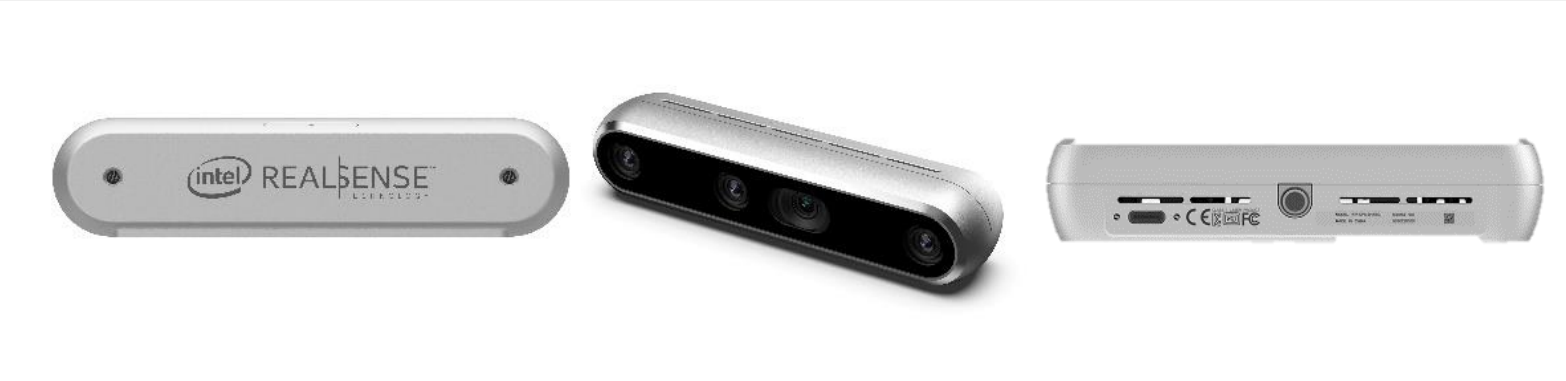
\includegraphics[width=0.9\textwidth]{figures/d455_example.png}
% 	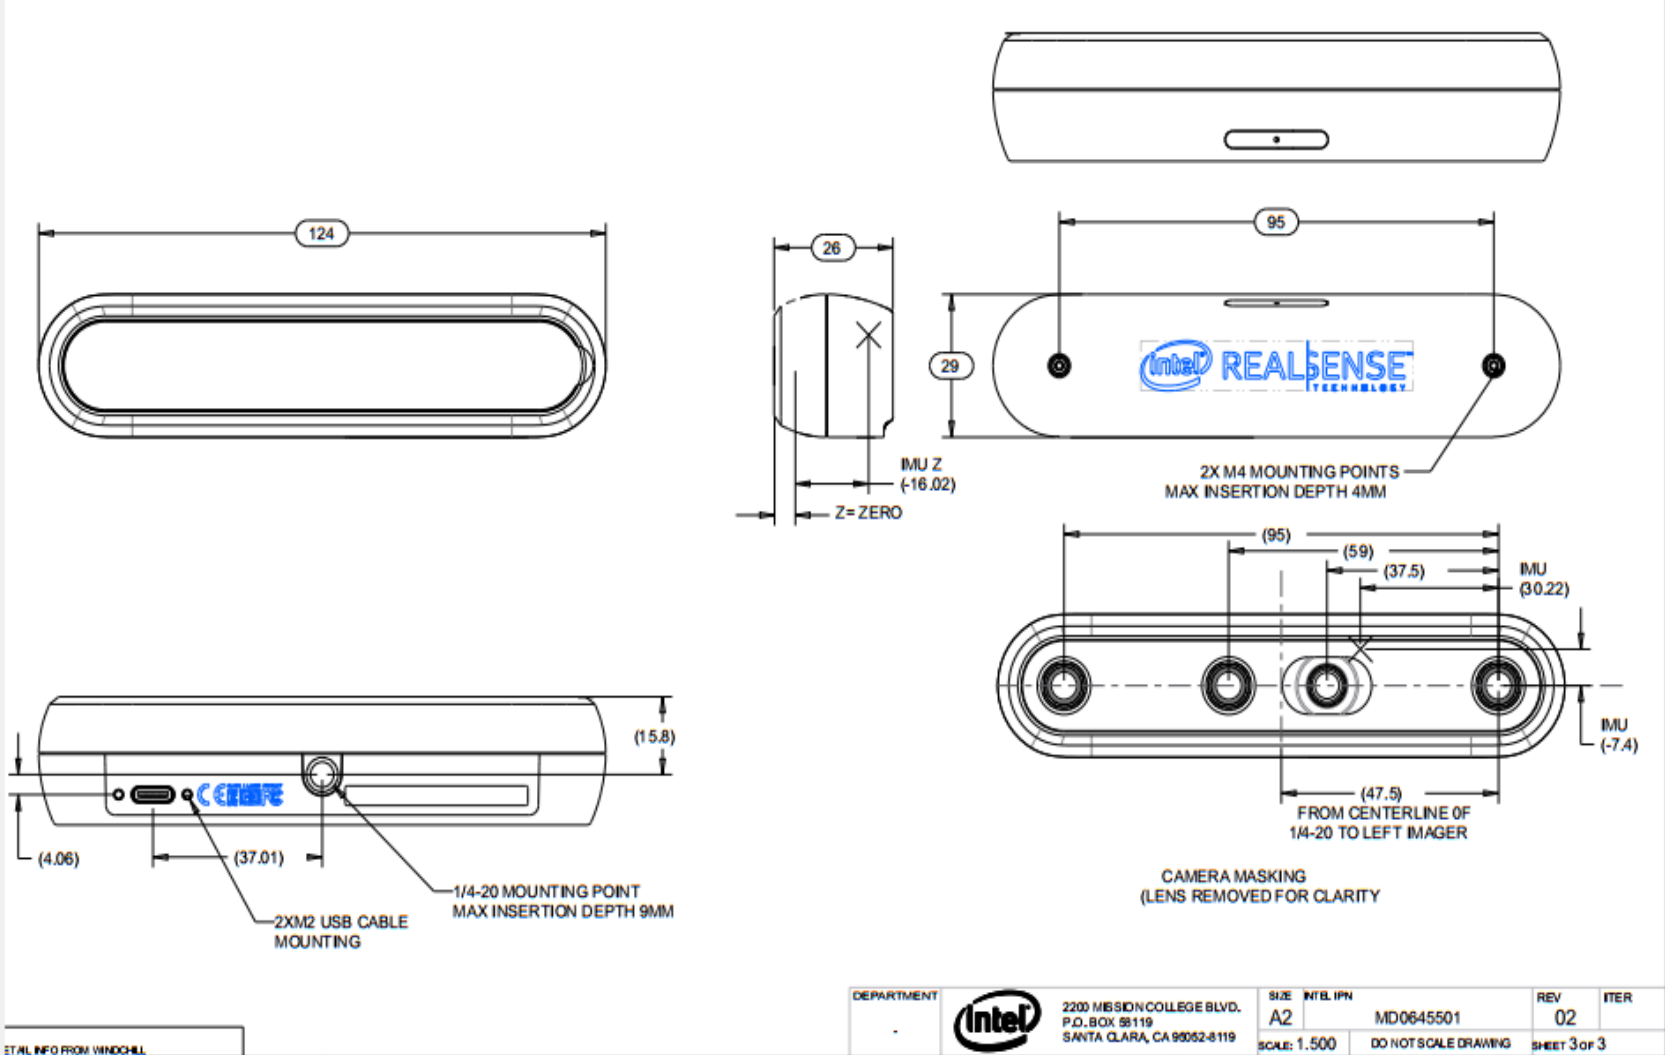
\includegraphics[width=0.9\textwidth]{figures/d455_structure.png}
% 	\caption{Intel ReadSense Depth Camera D455相机结构}
% 	\note{注:Intel RealSense Depth Camera D455 深度相机集成了一对立体深度传感器,一个RGB摄像头,以及一个内建的IMU惯性测量单元,摄像头的前面板标注有各种传感器和组件的名称和位置。该相机的每一个元素都设计得精巧紧凑,以提供高精度的深度感知能力,适应多种应用场景。}
% 	\label{fig:d455_example}
% \end{figure}
% \subsubsection{Intel ReadSense相机}

\par 在众多RGB-D相机品牌中,Intel RealSense 是一款备受欢迎的选择。Intel RealSense 由英特尔公司开发,具备实时3D扫描和物体识别功能,使设备能够与现实世界进行更自然、更直观的交互。
这款相机采用红外线投影仪和深度传感器捕捉物体的深度信息,实现场景的3D扫描和物体识别。同时,它能够捕捉高分辨率的RGB图像和深度图像,为用户提供丰富的视觉数据。
Intel
RealSense具有较高的计算性能,能够实时处理大量深度数据,为应用程序提供即时反馈。为了方便开发者快速集成RealSense技术,英特尔公司为其提供了一套全面的软件开发工具包(Software
Development Kit,SDK), 包括多种编程语言的应用程序接口(Application Program
Interface,API)、示例代码和文档等。此外,Intel
RealSense具有模块化设计,可根据不同的应用需求选择合适的模组进行组合,同时支持多种操作系统(如Windows、Linux、Android等),与各种硬件平台无缝集成。
目前,该型机的最新型号为Intel ReadSense Depth Camera
D455,技术规格见表~\ref{Intel_ReadSense_Depth_Camera_D455}。

\begin{table}[htb]
	\centering
	\caption{\href{https://www.intelrealsense.com/zh-hans/depth-camera-d455/}{Intel ReadSense Depth Camera D455 技术规格}}
	\label{Intel_ReadSense_Depth_Camera_D455}
	\begin{tabular}{c|ll}
		\toprule
		类型                   & \multicolumn{2}{c}{属性}                                                                                                                                    \\

		\midrule
		\multirow{2}{*}{特性}  & 使用环境:室内 / 室外                                                                        & 推荐范围:0.6 $\textasciitilde$ 6 m                                      \\
		                     & 深度快门类型:全局快门                                                                         & 惯性量测单元:Bosch BMI055                                                 \\

		\midrule
		\multirow{3}{*}{深度}  & 深度技术:立体                                                                             & 深度视场(FOV):\SI{87}{\degree} $\times$ \SI{58}{\degree}                \\
		                     & 最小深度距离 (Min-Z):$\textasciitilde$ 0.52 m                                             & 深度输出分辨率:高达 1280 $\times$ 720                                        \\
		                     & 深度精度< 2\%位于4 m                                                                      & 深度帧率:高达90帧/秒                                                        \\

		\midrule
		\multirow{3}{*}{RGB} & RGB帧分辨率:高达 1280 $\times$ 800                                                        & RGB 传感器 FOV (H \times V):\SI{90}{\degree} $\times$ \SI{65}{\degree} \\
		                     & RGB 帧速率:30 帧/秒                                                                      & RGB传感器分辨率:1 MP                                                      \\
		                     & RGB 传感器技术:全局快门                                                                      &                                                                     \\

		\midrule
		主要组件                 & 摄像头模块:英特尔实感模块 D450                                                                  & 计算处理器板:英特尔实感视觉处理器 D4                                                \\

		\midrule
		\multirow{3}{*}{物理}  & 外形:摄像头外设                                                                            & 接头:USB‑C* 3.1 Gen 1*                                                \\
		                     & \multicolumn{2}{l}{长度 $\times$ 深度 $\times$ 高度:124 mm $\times$ 26 mm $\times$ 29 mm}                                                                       \\
		                     & \multicolumn{2}{l}{安装机构:一个 1/4‑20 UNC 螺纹安装点、两个 M3 螺纹安装点、三脚架}                                                                                              \\

		\bottomrule
	\end{tabular}
	\note{注:深度精度是出厂测量值}
\end{table}

\par 在未来,RGB-D相机将会有很多可能的发展和改进方向。
为了满足更高精度和分辨率的需求,RGB-D 相机的硬件和算法将继续发展,未来会提供更高的深度精度,更细致的深度分辨率以及更低的噪声。
随着技术的进步,RGB-D相机将变得更小、更轻便,甚至被被集成到智能手机、平板电脑和其他便携式设备中\cite{alkhawaja_jaradat_romdhane_2023},这将进一步推动增强现实和虚拟现实的发展。
另一方面,为了在各种光照条件下保持良好的性能,RGB-D相机将会继续改进以克服环境干扰\cite{EfficientRGB-DSLAM},包括开发新的光学镜头、改进传感器技术以及设计更强大的算法以处理复杂环境中的数据。

\par 随着RGB-D相机技术的不断发展,它们将在新的应用领域得到广泛应用\cite{rgbd_ad,rgbd_respiratory}。
在未来,RGB-D相机的影响将不仅仅局限于影像采集和处理,更可能会改变我们与世界的交互方式。
\subsection{二维图像语义分割}

% \subsubsection{简介}

\par 对二维图像进行语义分割属于全景分割(Panoptic Segmentation,如图\ref{fig:panopticsegmentation})\cite{panopticsegmentation}的一部分,是计算机视觉领域的一项重要任务,
旨在将输入的二维图像中每个像素分配给特定的语义类别,如人、车、树等。这意味着对图像进行像素级别的分类和分割,使每个像素都被标记为属于图像中的哪个类别。
\begin{figure}[htbp]
	\centering
	\subfigure[RGB图像]{
		\begin{minipage}[t]{0.45\linewidth}
			\centering
			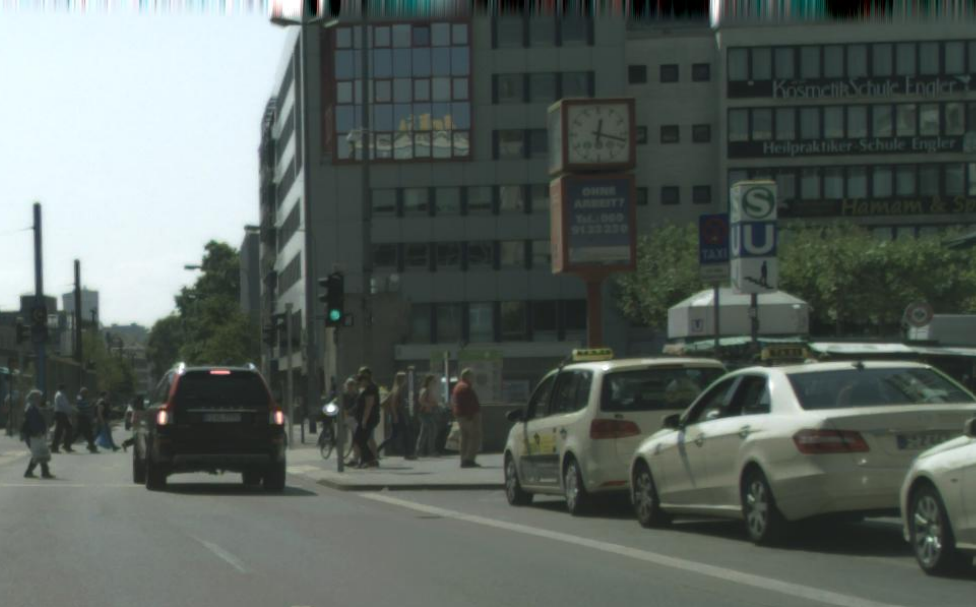
\includegraphics[height=4cm,keepaspectratio]{figures/panoptic_seg_1.png}
		\end{minipage}
	}
	\subfigure[语义图像]{
		\begin{minipage}[t]{0.45\linewidth}
			\centering
			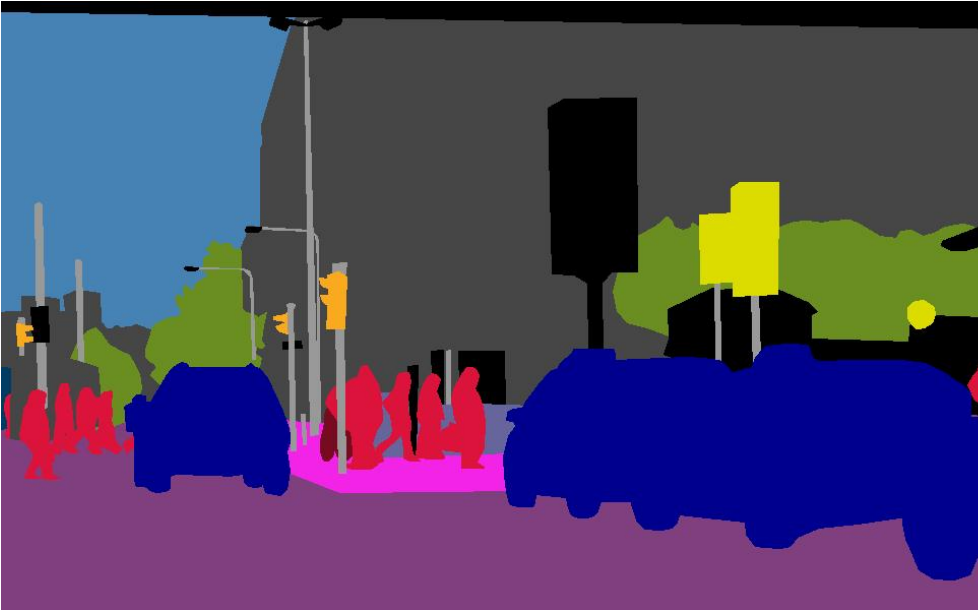
\includegraphics[height=4cm,keepaspectratio]{figures/panoptic_seg_2.png}
		\end{minipage}
	}

	\subfigure[实例图像]{
		\begin{minipage}[t]{0.45\linewidth}
			\centering
			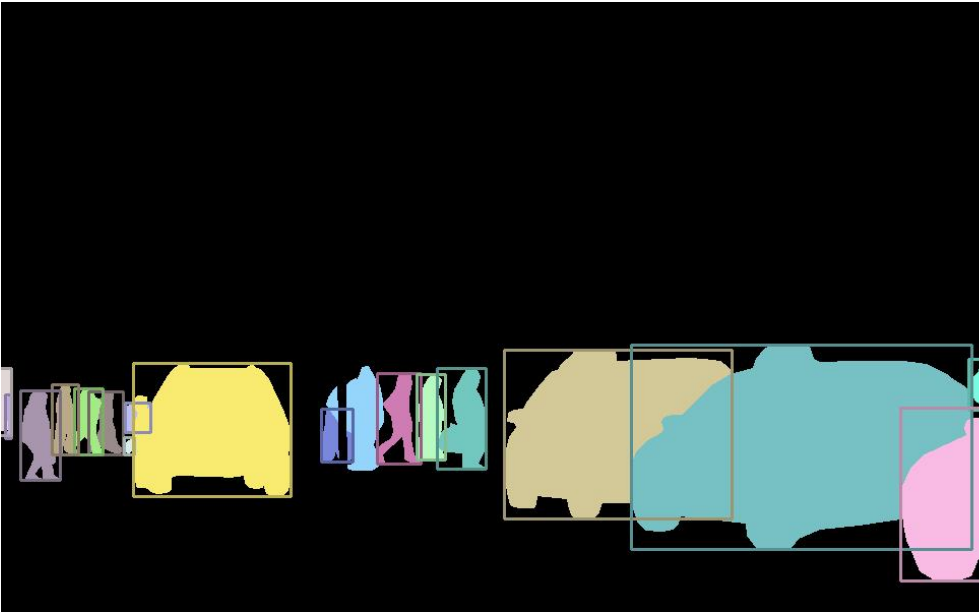
\includegraphics[height=4cm,keepaspectratio]{figures/panoptic_seg_3.png}
		\end{minipage}
	}
	\subfigure[全景图像]{
		\begin{minipage}[t]{0.45\linewidth}
			\centering
			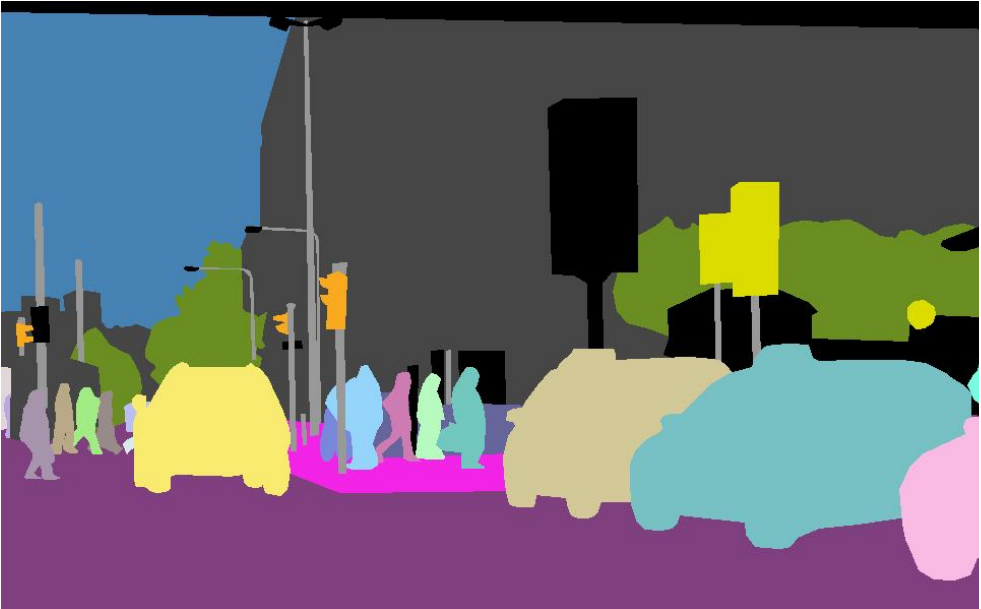
\includegraphics[height=4cm,keepaspectratio]{figures/panoptic_seg_4.png}
		\end{minipage}
	}
	\caption{二维图像全景分割}
	\label{fig:panopticsegmentation}
	\note{注:对于给定的RGB图像(a),(b)为语义分割,每个像素对应一个类别。(c)为实例分割,每个像素对应一个实例。(d)为全景分割。}
\end{figure}
语义分割对于自动驾驶、物体识别、场景理解等应用具有重要意义,可以为计算机系统提供更深入的关于图像内容的理解,为各种应用提供更准确和有用的信息。

% \subsubsection{研究现状}
\par 语义分割自从被提出以来,已经取得了显著的进展\cite{pascal,sift_flow,textonboost}。以下是截止2023年5月的一些研究现状:

\paragraph{SegNet}
\par 2015年,Vijay Badrinarayanan等人提出了SegNet\cite{segnet},这是一个基于编码器-解码器架构的深度学习模型。
SegNet的编码器网络对图像进行下采样以提取特征,然后解码器网络将这些特征图上采样回原始图像的大小,以进行像素级的分类。

\paragraph{Deeplab系列}
\par Deeplab\cite{deeplab}是一种高效的深度学习模型,它在语义分割任务中达到了很高的精度。Deeplab的主要创新是使用了空洞卷积(Dilated
Convolution)和条件随机场(Conditional Random Fields,CRF)。
空洞卷积可以在不增加计算复杂度的情况下增大感受野,而条件随机场可以改善分割结果的细节部分。后续的Deeplabv2\cite{deeplab2}、Deeplabv3
和 Deeplabv3+\cite{deeplab3plus}进一步提升了性能, 其中Deeplabv3引入了空洞空间金字塔池化模块(Atrous
Spatial Pyramid Pooling,ASPP)模块以捕获多尺度信息,Deeplabv3+
则加入了编码器-解码器结构,提升了分割的精度,如图\ref{fig:Deeplabv3+}\cite{deeplab3plus}所示。

\begin{figure}[htb]
	\centering
	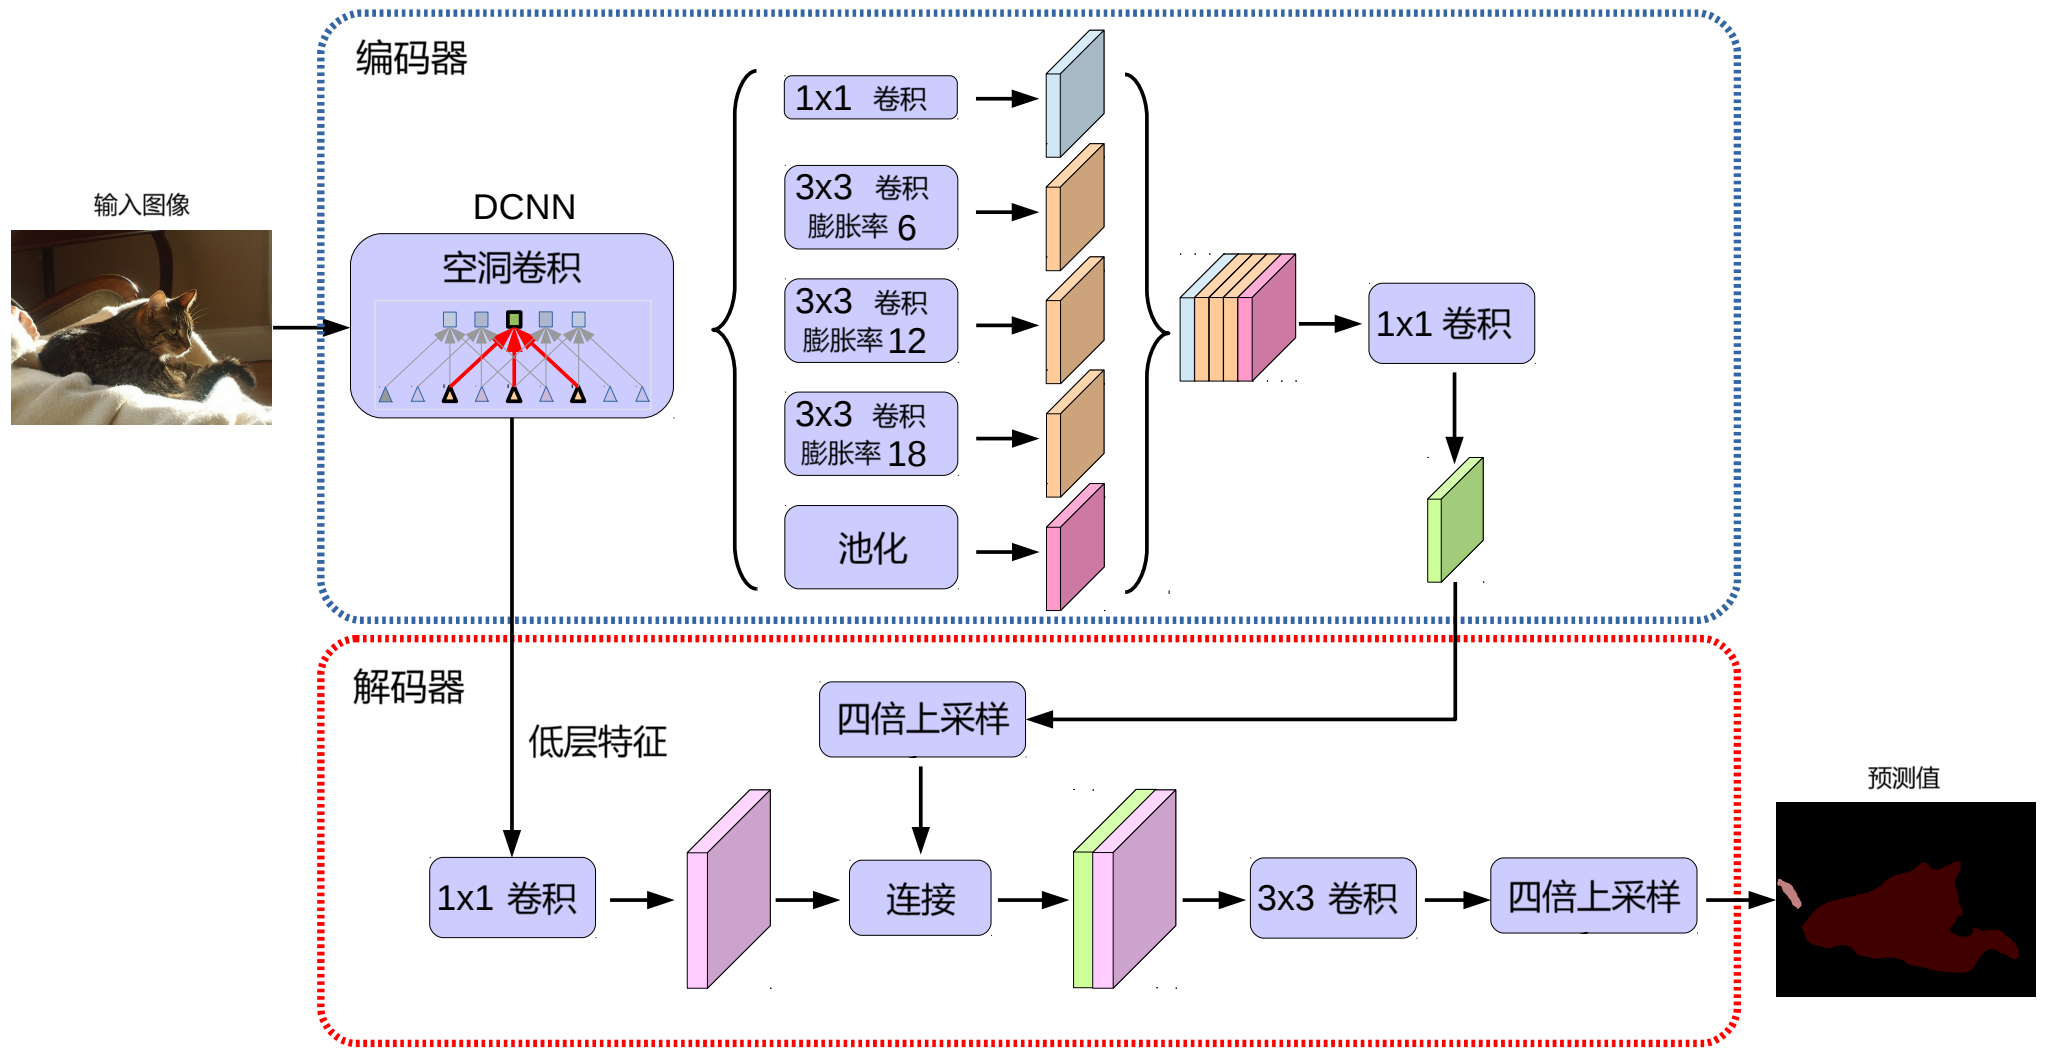
\includegraphics[width=0.9\textwidth]{figures/deeplab3_endecoder.png}
	\caption{Deeplabv3+的编码器-解码器结构}
	\label{fig:Deeplabv3+}
	\note{注:DeepLabv3+ 通过采用编码器-解码器结构扩展 DeepLabv3。其中,编码器通过在多个尺度应用空洞卷积实现编码多尺度上下文信息,而解码器则沿对象边界细化分割结果。}
\end{figure}

\paragraph{SAM}
\par SAM(Segment Anything Model)\cite{segment_anything}是由 Meta AI Research 开发,于 2023
年4月首次推出的一个模型,可用于分割图像中的任何对象。
该模型在图\ref{fig:sa-1b}\cite{segment_anything}所示的1100万张图像和11亿个掩码的大规模数据集SA-1B上进行训练,无需对新对象或图像进行额外的训练即可进行分割,生成高质量的分割掩码。
尽管 SAM 仍在开发过程中,但是它已经在各种场景中展示出巨大的应用潜力,有可能彻底改变我们与计算机和周围世界的互动方式。

\begin{figure}[htb]
	\centering
	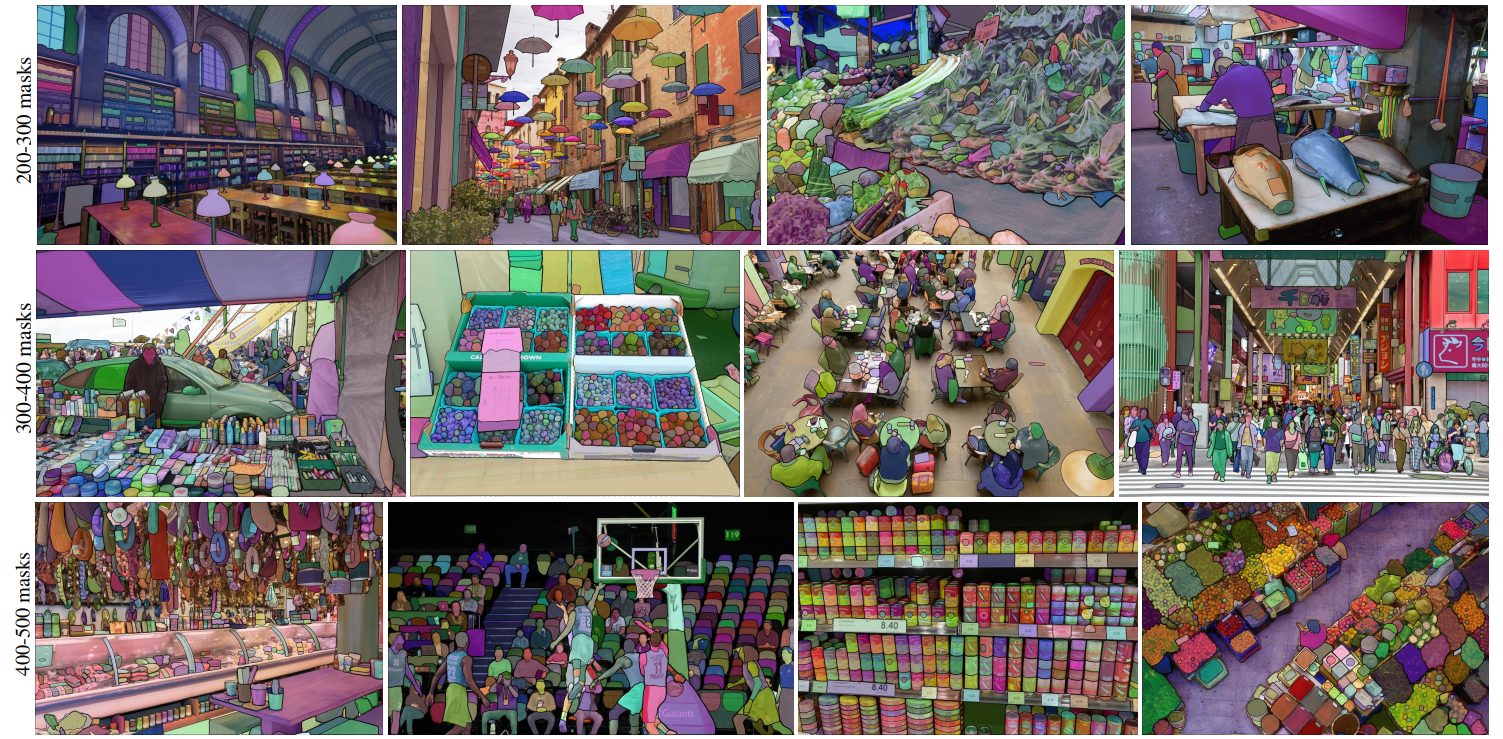
\includegraphics[width=0.9\textwidth]{figures/sam_result.png}
	\caption{SA-1B数据集示例图}
	\label{fig:sa-1b}
	\note{注:SA-1B数据集包含了1100万高质量、多样化的图片及11亿个精确分割蒙版示例。}
\end{figure}

\par 尽管语义分割已经取得了很大的进展,但它仍然面临着处理多尺度问题、减小计算复杂度和提高分割精度等挑战。
为了解决这些问题,未来的研究将主要集中在三个方向:
首先是端到端的训练方法\cite{pspnet,deeplab3plus}。这种方法可以一次性完成整个任务,提高了效率并且能够避免不一致的结果;
其次,随着计算机视觉技术的发展,语义分割被期待在嵌入式设备和实时应用中发挥更大的作用,这需要提高分割算法的效率和速度;
最后,多模态语义分割,即整合多种类型的输入数据,如雷达、激光雷达(LiDAR)或声音,将有助于提供更准确和更鲁棒的结果\cite{SceneParsing,CascadedPyramidNetwork}。
\subsection{三维重建}

\par 三维重建是一种将二维图像或者其它类型的数据转换为三维模型的技术。这个过程通常涉及到多个步骤和多种算法,
包括图像处理、特征检测、几何计算等。三维重建在许多领域都有应用,如医学成像、电影制作、虚拟现实和地理信息系统。
例如,在医学领域,可以从一系列的二维计算机断层扫描(Computerized Tomograph,CT)或磁共振成像(Magnetic Resonance Imaging,MRI)扫描图像中重建出三维的人体器官模型,
帮助医生更好地理解患者的病情。\cite{bushong2003magnetic,song2017review}在电影制作和游戏开发中,通过三维扫描和重建技术,可以把真实世界的人物或场景转换为三维模型,用于创造更逼真的视觉效果\cite{SLAMCast,hasenfratz2003survey,finance2015visual}。

\par 基于RGB-D相机的三维重建技术主要利用RGB图像信息和深度图像信息创建三维模型。
这种方法在处理复杂的场景时,比如有遮挡、自反射、各种材质和颜色的场景时,会有更好的效果\cite{SLAMCast,cavallari2019real,Dynamicfusion,Fusion4d},因为 RGB-D 相机提供的深度信息,可以直接用于计算物体的形状和位置,而不需要像传统的立体视觉那样进行复杂的深度计算。
在重建过程中,首先相机会捕捉一系列的 RGB-D 图像,然后通过“配准”的过程,将这些图像对齐在一起,创建一个一致的三维表示。
这个过程需要处理相机移动和旋转带来的视角变化。最后,利用“融合”的技术,将所有深度图像融合在一起,创建一个完整的三维模型。
这个过程需要处理噪声和不一致性,以保证三维模型的质量和准确性。

% \par 基于RGB-D相机的三维重建技术利用RGB图像和捕捉颜色信息,
% 利用深度图像技术物体表面到相机的距离,从而生成三维点云数据。
% 通过将这两种信息融合,可以精确地重建物体的几何形状和表面纹理。

\par 1996年,Curless 和 Levoy 首先提出了基于体素的重建方法\cite{VolumetricMethod},
通过使用一个规则网格来存储表示模型的离散化的符号距离函数(Signed Distance Function,SDF)。
该方法被Rusinkiewicz等人的首个实时重建算法\cite{rusinkiewicz2002real}和后来的
KinectFusion\cite{newcombe2011kinectfusion,izadi2011kinectfusion}采用。
基于体素的重建方法使用 SDF 隐式地存储模型表面,
即内部和外部体素分别存储到最近表面点的负距离和正距离,表面本身被定义为 SDF 的零交叉点,
在执行算法之前,必须定义体素的大小和网格的空间范围。
此外,每个体素中可以存储额外的属性信息,如颜色信息。

\par 常规的体素网格存储效率非常低,在实时场景重建时,大多数方法严重依赖 GPU 的处理能力,并且重建空间范围和分辨率通常受到 GPU 显存的限制。
为了支持更大的空间范围,不同学者已经提出了各种方法来提高基于体素的表示的存储效率\cite{whelan2016elasticfusion,vicini2021non,hornung2013octomap}。
为了防止在当前重建范围之外获取的深度图像而导致数据丢失,Whelan 等人
提出了一种简单的动态移动体素网格的方法\cite{whelan2012kintinuous},使其跟随相机的运动而运动。
该方法将移动到当前重建范围之外的部分体素转换为表面网格并单独存储。
虽然该方法可以实现更大的重建范围,但需要大量的离线内存使用,并且已经无法实时访问已重建完成并流出的表面。
\subsection{三维语义分割}

\par 三维语义分割是三维重建行业一个新的研究方向,其目标是将一个三维模型分割成不同的语义区域,通常涉及到两个步骤:首先,从一组图像中重建出三维场景;然后,应用一种分割算法,对每个三维点或体素进行语义标注。
目前,三维语义分割在计算机视觉和深度学习领域已经得到了广泛的研究。\cite{3DSemanticParsing,parislille3d}

\par 卷积神经网络(Convolutional Neural Network,CNN)和图神经网络(Graph Neural Network,GNN)已经在三维语义分割中得到了广泛的应用。例如,PointNet 和其后续版本 PointNet++\cite{pointnet,pointnet++} 使用 CNN 直接处理无序的点云数据,实现了有效的三维分割。
PointCNN\cite{PointCNN} 通过学习$\chi$变换,将无序的点云数据转换成带权重和潜在规范顺序的形式,从而在点云中实现类似传统 CNN 网络卷积操作的特征学习。
此外,一些工作使用 GNN 来处理三维空间的结构信息,以提升分割效果。

\par 为了进一步改善三维重建和语义分割的效果,近年来研究者提出了一些新的技术和方法。例如,PanopticFusion\cite{panopticfusion}首次提出实时地将全景分割图像整合到三维模型中。该方法通过贪心匹配算法将点云与图像中分割出的片段进行匹配,然后整合到TSDF点云模型中\cite{VolumetricMethod,voxblox},并且通过加权函数调整每个点对应的语义类别标签。其中,语义类别标签根据语义分割图像提供的置信度分数生成。此外,他们还应用了条件随机场(Conditional Random Field,CRF)来规范重建过程,从而提高了重建精度。在 PanopticFusion 的基础上,Voxblox 对深度图像进行分割来提高语义分割的准确性,使用几何分割结果和语义分割结果计算出成对权重(Pair-Wise Weight),用于点云类别标签的匹配。
 
\par 一些研究者基于 Voxblox 和 Voxblox++\cite{voxblox++},对三维重建语义融合的过程作出两个改进\cite{ReconstructingInteractive3D}:将类别标签加入到成对权重中,组合成三元权重(Triplet Weight);另外,如果语义分割图像中两个片段的重叠度达到一定阈值,则它们也会被融合。同时,他们还介绍了一种基于几何分割、语义分割和物理定律的方法,将CAD模型与重建物体进行对齐。该方法可以重建出接触图和交互式虚拟场景,使机器人与环境互动。

\par 在实时性方面,Online SegFusion\cite{OnlineSegFusion} 提出了一个基于深度神经网络的实时视觉框架,可以在重建出室内场景三维模型的同时进行语义融合更新。该方法放弃了在线深度融合中使用路由网络,使用涡流池化块(Vortex Pooling)保留高频表面细节,可以有效地融合语义标签和三维模型。

\par 尽管以上研究已经取得了显著的成果,但是在实时三维重建和语义分割领域,目前却仍然面临一些挑战。首先是实时处理大规模数据的问题。由于三维数据,尤其是点云数据,通常规模较大,因此处理这些数据需要大量的计算资源。虽然一些优化算法和多进程加速技术可以提高处理速度\cite{VoxelHashing,Real-TimeVolumetric,Multi-resolutionSurfaceReconstruction},但如何在保持高精度的同时实现实时处理仍然是一个挑战,需要使用更高级的算法和硬件资源(如 GPU)\cite{GPUAccelerated}。

\par 其次,虽然神经网络已经在三维分割中取得了很好的性能,但是如何有效地将语义信息融入到三维模型中仍然是一个难题。一方面,分割模型可能会产生错误或不确定的标签;另一方面,语义信息和几何信息可能会存在不一致性。解决这一问题需要更高级的语义融合算法。

\par 最后,动态环境的处理也是一个难题。环境中发生位移的物体会引入噪声和不一致性,影响三维重建和语义分割的精度\cite{VideoPanopticSegmentation}。解决这个问题需要系统能够增量式更新三维模型,这在技术上具有非常大的挑战性。

\par 这些挑战需要在算法、模型和硬件资源等多个方面进行创新和优化,以实现更好的实时三维重建和语义分割。

% 三维语义分割是三维重建行业一个新的研究方向,其目标是将一个三维模型分割成不同的语义区域,通常涉及到两个步骤:首先,从一组图像中重建出三 维场景;然后,应用一种分割算法,对每个三维点或体素进行语义标注。 目前三维语义分割在计算机视觉和深度学习领域已经得到了广泛的研究,它的研究现状和发展趋势具有以下特点: 

% (1)深度学习的广泛应用
% 深度学习,特别是卷积神经网络(convolutional neural network,CNN)和图神经网络(graph neural network,GNN),已经在三维语义分割中得到了广泛的应用。例如,PointNet 和其后续版本 PointNet++ 使用 CNN 直接处理无序的点云数据,实现了有效的三维分割。此外,一些工作使用 GNN 来处理三维空间的结构信息,以提升分割性能。 

% (2)全景数据的利用
% 为了捕获场景的全局信息,一些方法开始直接使用全景数据进行三维分割。 例如,一些工作将全景图像转换为球形投影或立方体投影,然后应用二维的深度学习方法进行分割。此外,一些工作结合全景视角和多视图技术,以提高重建和分割的精度。

% (3)大规模数据集的构建
% 大规模的标注数据集对于训练深度学习模型至关重要。例如,ScanNet 和 Matterport3D等数据集提供了大量的室内场景的三维扫描和语义标注, 推动了三维分割的研究。然而,构建这样的数据集需要大量的手工标注, 因此自动或半自动的标注方法是一个重要的研究方向。

% 但是,在实时三维重建和语义分割方面,三维语义分割正在面临一些挑战:

% 首先是实时处理大规模数据的问题。由于三维数据,尤其是点云数据,通常规模较大,因此处理这些数据需要大量的计算资源。虽然一些优化算法和多进程加速技术可以提高处理速度,但如何在保持高精度的同时实现实时处理仍然是一个挑战,需要使用更高级的算法和硬件资源(如 GPU)。

% 其次,尽管深度学习已经在三维分割中取得了很好的性能,但是如何有效地将语义信息融入到三维模型中仍然是一个难题。一方面,分割模型可能会产生错误或不确定的标签;另一方面,语义信息和几何信息可能会存在不一致性。

% 最后,动态环境的处理也是一个难题。环境中发生位移的物体会引入噪声和不一致性,影响三维重建和语义分割的精度。解决这个问题需要系统能够增量式更新三维模型,这在技术上具有非常大的挑战性。

% 这些挑战需要在算法、模型、和硬件资源等多个方面进行创新和优化,以实现更好的实时三维重建和语义分割。 

\section{论文主要内容及创新点}

% \par 本文设计并实现了基于RGB-D相机的实时三维重建及语义分割系统,
% 主要研究内容如下:
% \begin{enumerate}
%     \item 探讨三维重建及语义分割系统的开发背景及开发意义,调研国内外相似系统和有关算法的研究现状及发展趋势。之后,在调研结果的基础上,结合系统使用场景和使用平台,总结出系统需要具备的功能性需求和非功能性需求。
%     \item 根据需求分析的结果,采用模块化设计、数据驱动和层次化功能划分等设计方法,将系统所需具备的功能分别用数据采集模块、点运生成与语义融合模块、可视化模块等模块进行实现,并且在此基础上将系统划分为硬件层、系统交互层、预处理层、核心算法层和表现层,以提高系统的灵活性和可扩展性。此外,对每个模块的执行流程和数据类型进行了具体的设计。
%     \item 对系统各个模块进行详细设计,使用类图、时序图、类表、伪代码、数学公式等方法阐述实现细节。
%     \item 对系统进行测试。首先,根据功能性需求和非功能性需求确定使用的测试指标,设计特定的测试用例。其次,根据测试用例对各个模块和整个系统进行全面的测试,以验证系统能否满足各项需求。
% \end{enumerate}

\par 本文设计并实现了基于RGB-D相机的实时三维重建及语义分割系统,本人的主要工作是系统中数据预处理、场景管理、点云生成、实时语义融合与更新、可视化、滤波降噪以及模型导入导出功能的开发,实现了根据给定的RGB-D图像、语义分割图像和相机位姿矩阵,生成并交互具有语义信息的三维点云模型的全部过程。

\par 本文将语义融合、更新的过程转化为线性分配问题,与点云生成过程分离,有效解决了对动态范围场景进行实时性、增量式重建的难题。
本文提出使用重叠空间网格的方法,对动态场景空间进行划分,提高了重建的灵活性和效率。
此外,系统全面使用GPU进行点云生成和语义融合更新的计算,显著提高了处理速度。
这些创新使得系统可以应用于室内重建、工业生产及自动驾驶等多个场景。

\section{论文组织结构}
\paragraph{第1章:绪论}
\par 本章首先介绍了研究的背景和研究意义,探讨了RGB-D相机技术、二维图像全景分割、三维重建和三维语义分割前沿领域的研究现状。接着概述了论文的主要内容和本人的工作,明确了论文的目标和贡献。

\paragraph{第2章:关键技术}
\par 本章详细介绍了支撑系统的关键技术,从相机位姿估计、深度学习模型、三维重建算法到GPU架构、图形渲染等方面进行了阐述,为后续系统设计和实现提供了必要的背景知识。

\paragraph{第3章:实时三维重建及语义分割系统需求分析}
\par 本章从系统概述的角度出发,明确了系统的功能性需求和非功能性需求。通过系统化的分析,为后续的系统设计提供了明确的指导,确保系统满足设计和应用的期望。

\paragraph{第4章:实时三维重建及语义分割系统概要设计}
\par 本章从整体架构和模块设计两个层面进行系统的设计。通过分析各个模块的功能和相互关系,为系统的实现奠定了基础。

\paragraph{第5章:实时三维重建及语义分割系统详细设计与实现}
\par 本章进一步深入,详细描述了系统各个模块的设计和实现过程。对于数据采集、位姿估计、语义分割、点云生成等关键模块进行了逐一分析和阐述。同时,展示了系统的实现效果。

\paragraph{第6章:系统测试}
\par 本章对实现后的系统进行了测试,介绍了测试所使用的数据集和评价指标,明确了测试方案和用例。通过单元测试和集成测试,验证了系统在不同层次上的性能表现。

\paragraph{第7章:总结与展望}
\par 本章对整个系统设计与实现进行了总结,回顾了已经实现的系统功能和创新点,同时展望未来可能的研究方向和改进空间。

\paragraph{其他}
\par 附录部分提供了一些补充材料,如项目源代码、系统运行动画、语义分割正确率等,以增强读者对于论文工作的理解和验证。最后,感谢所有对本论文的支持和帮助,并在参考文献中列出了相关的学术资料和技术文档。